\section{COUPLED FIELDS ANALYSIS} \label{ch_5.4}
\normalsize{In the above chapter, it was concluded that complex coupled phenomena such as temperature and displacement dependant contacts. To understand the coupling method and its mathematical implications, a little introduction to coupling will be done.}
\subsection{Introduction to coupled fields analysis}
\normalsize{There are many different methods for multiphysics coupling. This idea of coupling fields is to consider the effect of field A on field B and vice-versa using coupling terms.}
\\
\begin{figure}[!ht]
    \label{fig_5_21}
    \centering
    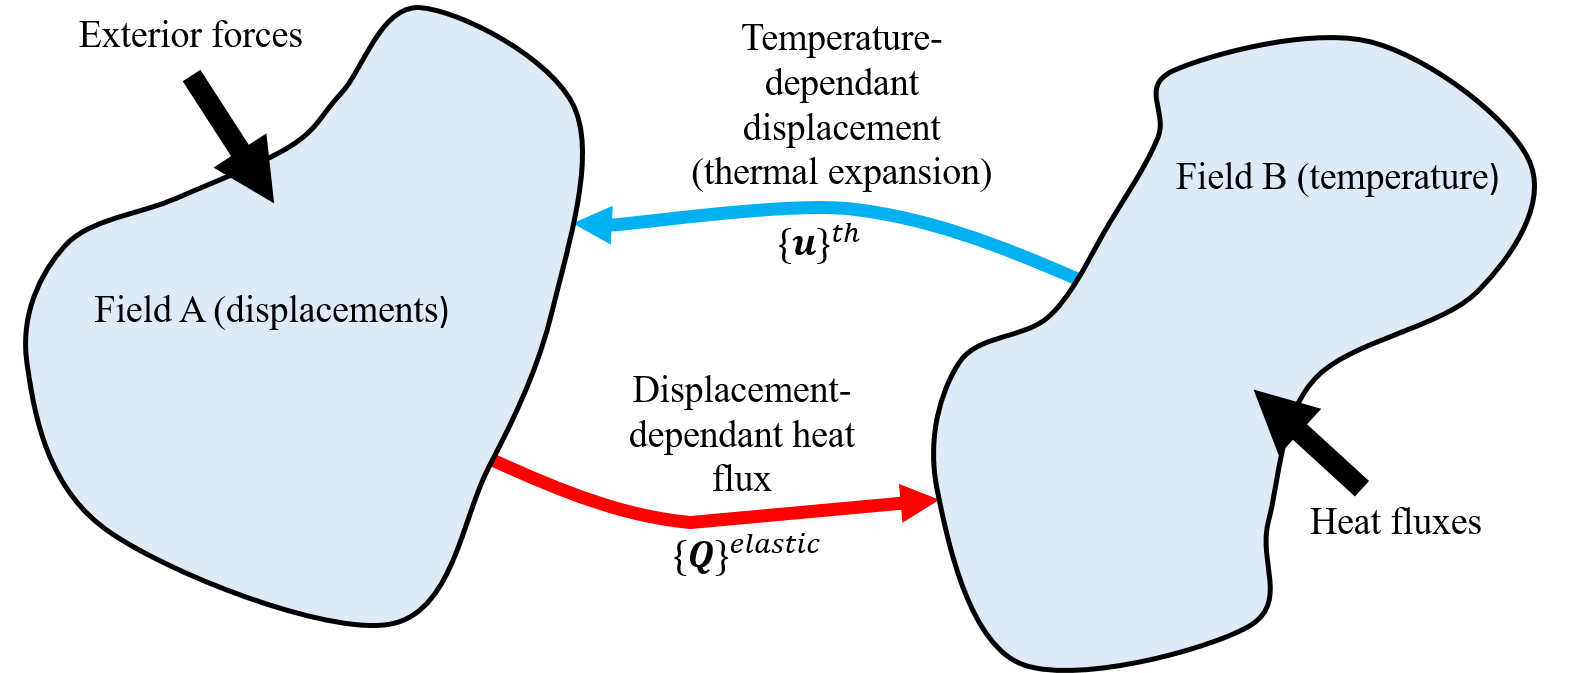
\includegraphics[width=1\textwidth]{figures/patateCoupling.png}
    \caption{\it Fields coupling.}
\end{figure}
\\
\normalsize{The coupling can be made of two different levels, the weak coupling (vector coupling) and the strong coupling (matrix coupling). The vector coupling is generally less computationally expensive. It works by adding to the right-hand side of the equation a coupling vector.}
\\

\begin{equation}
    \begin{bmatrix} K[1,1] & 0 \\ 0 & K[2,2] \end{bmatrix}
    \begin{Bmatrix} \{Displacement \ field\} \\ \{Temperature \ field\} \end{Bmatrix}
    =
    \begin{Bmatrix} \{Forces\}+\{Forces\}_{thermal} \\ \{Heat \ fluxes\}+\{Heat \ fluxes\}_{th. elastic} \end{Bmatrix}
    \label{eq:coupling}
\end{equation}
\\
\normalsize{\indent This method is less computationally expensive since the coupling is done ba adding the coupling vector. The system matrix is diagonal, meaning that it is possible to decouple the calculation of the displacement field and the temperature field and create two subproblems such that:}
\\
\begin{equation}
    K[1,1] \{Displacement \ field\} = \{Forces\}+\{Forces\}_{thermal}
\end{equation}
\normalsize{and the other}
\begin{equation}
    K[2,2] \{Temperature \ field\} = \{Heat \ fluxes\}+\{Heat \ fluxes\}_{th. \ elastic}
\end{equation}
\\
\normalsize{\indent This also means that the fields are NOT calculated at the same time but rather one after the other. The method while taking less storage space requries more steps. Another way to couple the fields is using the strong coupling (matrix coupling). In this method, the fields are not longer coupled using a coupling vector but rather directly in the system matrix by introducing off-diagonal coupling terms {\bfseries K[1,2]} and {\bfseries K[2,1]}. Those terms allows a direct coupling of the fields as well as simultaneous calculations of the solution vector. This method is computationally expensive and will require more storage space but less steps.}
\\
\begin{equation}
    \begin{bmatrix} K[1,1] & K[1,2] \\ K[2,1] & K[2,2] \end{bmatrix}
    \begin{Bmatrix} \{Displacement \ field\} \\ \{Temperature \ field\} \end{Bmatrix}
    =
    \begin{Bmatrix} \{Forces\} \\ \{Heat \ fluxes\} \end{Bmatrix}
    \label{eq:coupling3}
\end{equation}
\\
\normalsize{\indent Weak coupling is the method used in this analysis because the model is not complex, the contact surfaces are plane and the bolting system is not modelled. The preload of the bolts is modelled using forces. Those forces were derived from previous structural only analysis (in average the preload force is 750 \unit{W}). A comparison with strong coupling \ref{eq:coupling3} was done to assess the result differences and the results showed little deviation.}
\subsection{Static thermal-structural analysis of the tile assembly}
\normalsize{After these considerations, it is possible to proceed with the calculations. The model is tested for four load cases \ref{table:scenarios}.}
\\
\begin{figure}[!ht]
    \label{fig_5_22}
    \centering
    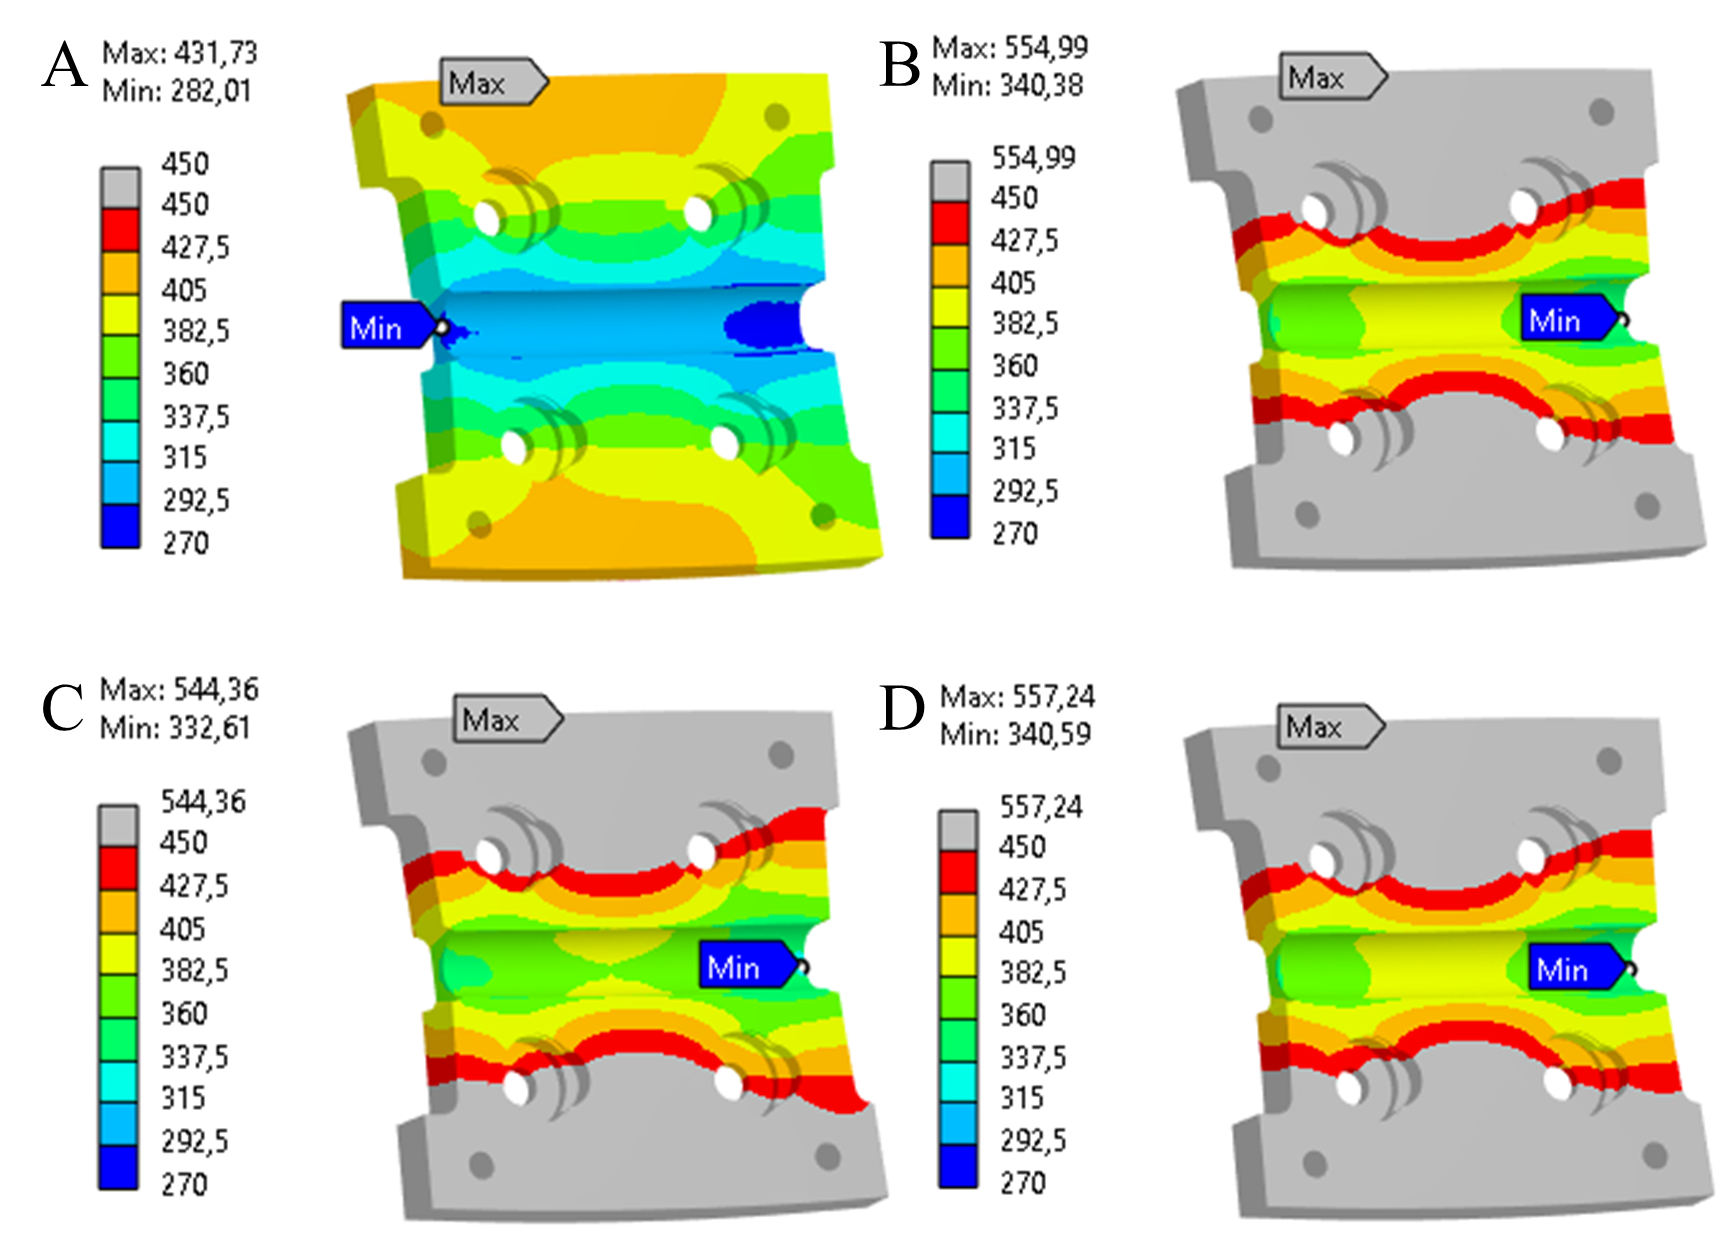
\includegraphics[width=1\textwidth]{figures/multiphysicsResults.png}
    \caption{\it Coupled analysis of \acrshort{CuCrZr} heat sink per load case. A is plasma heat load only, B is plasma heat load + ECRH axisymmetric heat load, C is plasma heat load + ECRH non-axisymmetric heat load, D is plasma heat load + ECRH axisymmetric heat load (J. Zhu parameters) \cite{zhu_parametric_2019}.}
\end{figure}
\\
\normalsize{\indent The results are showing high \acrshort{CuCrZr} temperatures. The maximum temperatures are higher for the coupled analysis compared to the case with 100 \% of thermal contact and the manually updated contact. It is possible to compare with a table to get a more direct comparison.}
\\
\break
\normalsize{\indent While the coupled analysis can be more handy when it comes to modelling complex phenomena, they are quite complex to set up. The problem of the contact configuration plagued the model by conditionning the problem is such a manner that it becomes unstable and won't properly converge for all \acrshort{DoF}s. This is the reason why, for this early multiphysics model, the bolting system had to be excluded.}
\\
\begin{table*}[h!]
    \centering
    \ra{1.3}
    %\begin{tabular}{@{}cccc@{}}
    \begin{tabular}{p{3,8cm}p{2cm}p{2,4cm}p{2cm} }
    \toprule
    $Load \ cases$ & $Full \ contact$ & $Reduced \ contact$ & $Full \ coupling$ \\
    \cmidrule{1-4}

    Plasma heat load (250 \unit{kWm^{-2} }) & $414,24$ & $406,26$ & $431,73$\\
    \myrowcolour
    Plasma heat load + \acrshort{ECRH} axisym. & $511,67$ & $494,63$ & $554,99$\\
    Plasma heat load + \acrshort{ECRH} non-axisym. & $503,85$ & $487,64$ & $544,36$\\
    \myrowcolour
    Plasma heat load + \acrshort{ECRH} non-axisym. (J. Zhu param.) & $515,88$ & $496,39$ & $557,24$\\

    % \midrule
\bottomrule
\end{tabular}
\caption{Temperature table of the \acrshort{CuCrZr} heat sink per load case vs. modelling method in \unit{\si{\degree}C}. }
\end{table*}
\\
\normalsize{\indent This table gives insight about the different results, namely, the fact that the coupled analysis will produce much higher maximum temperatures. The results are particularly conservative and better material propoerties could have predicted different temperatures. For the Plasma heat load + \acrshort{ECRH} axisymmetric load case the temperature increased by about 10 \% (ref. full contact calculations). For the Plasma heat load + \acrshort{ECRH} non-axisymmetric loadcase: temperature increased by about 9,5 \% (ref. full contact calculations). When \acrshort{ECRH} load is applied, large volumes of the heat sink exceed the limit temperature (if max. temperature is 450 \si{\degree}C) ($24,8 \%$ of the temperature limit for Plasma heat load + \acrshort{ECRH} axisymmetric loadcase and $22,5 \%$ of the temperature limit for Plasma heat load + \acrshort{ECRH} non-axisymmetric loadcase.) }
\\
\break
\normalsize{These results show that the optimal way to model the tile assembly and to perform optimal calculations, {\bfseries it is recommended to used a coupled physics model.} Multiphysics coupling including the bolting system but also including metallurgical phase change could be of use to get information about the state of the different parts during the life cycle of the assembly.}